\documentclass[12pt]{report}
\usepackage[utf8]{inputenc}
\usepackage[russian]{babel}
%\usepackage[14pt]{extsizes}
\usepackage{listings}
\usepackage{graphicx}
\usepackage{amsmath,amsfonts,amssymb,amsthm,mathtools} 
\usepackage{pgfplots}
\usepackage{filecontents}
\usepackage{float}
\usepackage{indentfirst}
\usepackage{eucal}
\usepackage{enumitem}
\frenchspacing

\usepackage{indentfirst} % Красная строка


\usetikzlibrary{datavisualization}
\usetikzlibrary{datavisualization.formats.functions}

\usepackage{amsmath}




% Для листинга кода:
\lstset{ %
language=haskell,                 % выбор языка для подсветки (здесь это С)
basicstyle=\small\sffamily, % размер и начертание шрифта для подсветки кода
numbers=left,               % где поставить нумерацию строк (слева\справа)
numberstyle=\tiny,           % размер шрифта для номеров строк
stepnumber=1,                   % размер шага между двумя номерами строк
numbersep=5pt,                % как далеко отстоят номера строк от подсвечиваемого кода
showspaces=false,            % показывать или нет пробелы специальными отступами
showstringspaces=false,      % показывать или нет пробелы в строках
showtabs=false,             % показывать или нет табуляцию в строках
frame=single,              % рисовать рамку вокруг кода
tabsize=2,                 % размер табуляции по умолчанию равен 2 пробелам
captionpos=t,              % позиция заголовка вверху [t] или внизу [b] 
breaklines=true,           % автоматически переносить строки (да\нет)
breakatwhitespace=false, % переносить строки только если есть пробел
escapeinside={\#*}{*)}   % если нужно добавить комментарии в коде
}

\usepackage[left=2cm,right=2cm, top=2cm,bottom=2cm,bindingoffset=0cm]{geometry}
% Для измененных титулов глав:
\usepackage{titlesec, blindtext, color} % подключаем нужные пакеты
\definecolor{gray75}{gray}{0.75} % определяем цвет
\newcommand{\hsp}{\hspace{20pt}} % длина линии в 20pt
% titleformat определяет стиль
\titleformat{\chapter}[hang]{\Huge\bfseries}{\thechapter\hsp\textcolor{gray75}{|}\hsp}{0pt}{\Huge\bfseries}


% plot
\usepackage{pgfplots}
\usepackage{filecontents}
\usetikzlibrary{datavisualization}
\usetikzlibrary{datavisualization.formats.functions}

\begin{document}
%\def\chaptername{} % убирает "Глава"
\thispagestyle{empty}
\begin{titlepage}
	\noindent \begin{minipage}{0.15\textwidth}
	
\includegraphics[width=\linewidth]{img/b_logo}
	\end{minipage}
	\noindent\begin{minipage}{0.9\textwidth}\centering
		\textbf{Министерство науки и высшего образования Российской Федерации}\\
		\textbf{Федеральное государственное бюджетное образовательное учреждение высшего образования}\\
		\textbf{~~~«Московский государственный технический университет имени Н.Э.~Баумана}\\
		\textbf{(национальный исследовательский университет)»}\\
		\textbf{(МГТУ им. Н.Э.~Баумана)}
	\end{minipage}
	
	\noindent\rule{18cm}{3pt}
	\newline\newline
	\noindent ФАКУЛЬТЕТ $\underline{\text{«Информатика и системы управления»}}$ \newline\newline
	\noindent КАФЕДРА $\underline{\text{«Программное обеспечение ЭВМ и информационные технологии»}}$\newline\newline\newline\newline\newline
	
	
	\begin{center}
		\noindent\begin{minipage}{1.3\textwidth}\centering
			\Large\textbf{  Отчет по лабораторной работе No4}\newline
			\textbf{по дисциплине "Операционные системы"}\newline\newline
		\end{minipage}
	\end{center}
	
	\noindent\textbf{Тема} $\underline{\text{Процессы. Системные вызовы fork() и exec()}}$\newline\newline
	\noindent\textbf{Студент} $\underline{\text{Каримзай А-Х.~~~~~~~~~~~~~~~~~~~~~~~~~~~~~~~~~~~~~~}}$\newline\newline
	\noindent\textbf{Группа} $\underline{\text{ИУ7и-55Б~~~~~~~~~~~~~~~~~~~~~~~~~~~~~~~~~~~~~~~~~~~~~~}}$\newline\newline
	\noindent\textbf{Оценка (баллы)} $\underline{\text{~~~~~~~~~~~~~~~~~~~~~~~~~~~~~~~~~~~~~~~~~~~~~}}$\newline\newline
	\noindent\textbf{Преподаватели} $\underline{\text{Рязанова Н.Ю.~~~~~~~~~~~~~~~~~~~~~~~~~~}}$\newline\newline\newline
	
	\begin{center}
		\vfill
		Москва~---~\the\year
		~г.
	\end{center}
\end{titlepage}

\newpage

\section*{Задание No1}

Процессы-сироты. В программе создаются не менее двух потомков. В потомках вызывается sleep(). Чтобы предок гарантированно завершился раньше своих помков. Продемонстрировать с помощью соответствующего вывода информацию об идентификаторах процессов и их группе.

\begin{lstlisting}[label=some-code,caption=Процессы-сироты,language=C]
#include <stdio.h>
#include <unistd.h>
#include <sys/types.h>>

#define REP_N 2 // loop rep time
#define SLP_T 2 // sleep time

enum error_code
{
    ok,
    error
};

int main()
{
    int child[REP_N];

    printf("Parent process PID = %d, Group: %d\n", getpid(), getpgrp());

    for (size_t i = 0; i < REP_N; i++) {
        pid_t pid = fork();

        if (pid == -1) {
            perror("Can't fork!");
            return error;
        } else if (pid == 0) {
            sleep(SLP_T);
            printf("\nChild process PID = %d, PPID = %d, , Group: %d\n", \
                                    getpid(), getppid(), getpgrp());
            return ok;
        } else {
            child[i] = pid;
        }

    }
    puts("msg from parent process");
    
    for (size_t i = 0; i < REP_N; i++)
        printf("child[%zu].pid = %d\n", i, child[i]);
    
    return ok;
}
\end{lstlisting}

\begin{figure}[H]

	\centering

	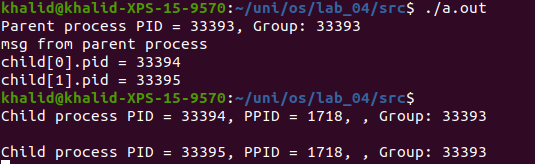
\includegraphics[width=\linewidth]{img/task01.png}
	\caption{Демонстрация работы программы (задание No1).}

	\label{fig:task01}

\end{figure}

\section*{Задание No2}

Предок ждет завершения своих потомком, используя системный вызов
wait(). Вывод соответствующих сообщений на экран.

\begin{lstlisting}[label=some-code,caption=Вызов функции wait(),language=C]
#include <stdio.h>
#include <unistd.h>
#include <sys/types.h>
#include <sys/wait.h>

#define REP_N 2 // loop rep time
#define SLP_T 2 // sleep time

enum error_code {
    ok,
    error
};

int main()
{
    int child[REP_N];
    

    printf("Parent process PID = %d, Group: %d\n", getpid(), getpgrp());

    for (size_t i = 0; i < REP_N; i++) {
        pid_t pid = fork();

        if (pid == -1) {
            perror("Can't fork!");
            return error;
        } else if (pid == 0) {
            sleep(SLP_T);
            printf("\nChild process PID = %d, PPID = %d, , Group: %d\n", \
                                    getpid(), getppid(), getpgrp());
            return ok;
        } else {
            child[i] = pid;
        }

    }
    puts("msg from parent process");
    
    for (size_t i = 0; i < REP_N; i++) {
        int status, ret_val = 0;
        
        pid_t child_pid = wait(&status);

        printf("\nChild process PID = %d, completed, status %d\n", \
                                    child_pid, status);
        
        if (WIFEXITED(ret_val))
            printf("Child process [No = %zu] completed with %d exit code\n", 
                                        i + 1, WEXITSTATUS(ret_val));
        else if (WIFSIGNALED(ret_val))
            printf("Child process [No = %zu] completed with %d exit code\n", 
                                        i + 1, WTERMSIG(ret_val));
        else if (WIFSTOPPED(ret_val))
            printf("Child process [No = %zu] completed with %d exit code\n", 
                                        i + 1, WSTOPSIG(ret_val));
    }
    
    puts("msg from parent process");
    
    for (size_t i = 0; i < REP_N; i++)
        printf("child[%zu].pid = %d\n", i, child[i]);

    return ok;
}
\end{lstlisting}

\begin{figure}[H]

	\centering

	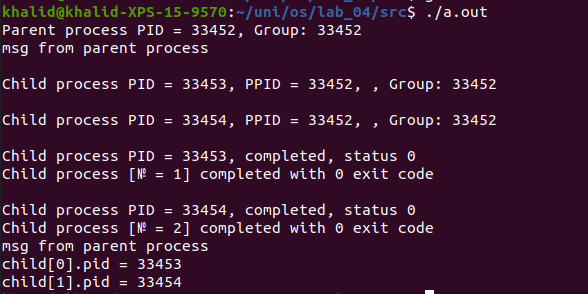
\includegraphics[width=\linewidth]{img/task02.png}
	\caption{Демонстрация работы программы (задание No2).}

	\label{fig:task02}

\end{figure}

\section*{Задание No3}

Потомки переходят на выполнение других программ. Предок ждет завершения своих потомков. Вывод соответствующих сообщений на экран.

\begin{lstlisting}[label=some-code,caption=Вызов функции execvp(),language=C]
#include <stdio.h>
#include <unistd.h>
#include <sys/wait.h>
#include <sys/types.h>

#define REP_N 2 // loop rep time
#define SLP_T 2 // sleep time

enum error_code {
    ok,
    error
};

int main()
{
    int child[REP_N];
    char *const args[4] = { NULL };
    char *const s_args[4] = { NULL };
    int pid;

    printf("Parent process PID = %d, Group: %d\n", getpid(), getpgrp());

    for (size_t i = 0; i < REP_N; i++) {
        pid = fork();

        if (pid == -1) {
            perror("Fork failed!");
            return error;
        } else if (pid == 0) {
            printf("\nChild process PID = %d, PPID = %d, Group: %d\n", \
                        getpid(), getppid(), getpgrp());
            
            int res;
            if (i == 0)
                res = execvp("/home/khalid/Desktop/c_labs/rk_03/a.out", args);
            else
                res = execvp("/home/khalid/Desktop/c_labs/rk_04/a.out", args);
            
            if (res == -1) {
                perror("exec failed!");
                return error;
            }
            
            return ok;
        } else {
            wait(NULL);
            child[i] = pid;
        }
    }

    puts("msg from parent process");
    
    for (size_t i = 0; i < REP_N; i++) {
        int status, ret_val = 0;
        
        pid_t child_pid = wait(&status);

        printf("\nChild process PID = %d, completed, status %d\n", \
                                    child_pid, status);
        
        if (WIFEXITED(ret_val)) {
            printf("Child process [No = %zu] completed with %d exit code\n", 
                                        i + 1, WEXITSTATUS(ret_val));
        } else if (WIFSIGNALED(ret_val)) {
            printf("Child process [No = %zu] completed with %d exit code\n", 
                                        i + 1, WTERMSIG(ret_val));
        } else if (WIFSTOPPED(ret_val)) {
            printf("Child process [No = %zu] completed with %d exit code\n", 
                                        i + 1, WSTOPSIG(ret_val));
        }
    }
    
    puts("msg from parent process");
    
    for (size_t i = 0; i < REP_N; i++)
        printf("child[%zu].pid = %d\n", i, child[i]);
    
    return ok;
}
\end{lstlisting}


\begin{lstlisting}[label=some-code,caption=код запушеного программа.,language=C]
#include <stdio.h>
#include <math.h>
#include <stdlib.h>

typedef struct
{
    int rows;
    int cols;
    int **mat;
} matrix;

enum error_code
{
    ok,
    error
};

matrix *create_matrix(const size_t rows, const size_t cols)
{
    matrix *tmp = malloc(sizeof(matrix));
    if (tmp)
    {
        tmp->rows = rows;
        tmp->cols = cols;
        tmp->mat = malloc(rows * sizeof(int *) + rows * cols * sizeof(int));
        if (tmp->mat)
        {
            for (int i = 0; i < rows; i++)
                tmp->mat[i] = (int *)((char *) tmp->mat + rows * sizeof(int *) + i * cols * sizeof(int));
        }
        else
        {
            free(tmp);
            tmp = NULL;
        }
    }
    return tmp;
}

void display_mat(matrix *mat)
{
    for (int i = 0; i < mat->rows; i++)
    {
        for (int j = 0; j < mat->cols; j++)
            printf("%5d ", mat->mat[i][j]);
        printf("\n");
    }
}

int fill_mat(matrix *mat)
{
    int x;
    for (int i = 0; i < mat->rows; i++)
    {
        for (int j = 0; j < mat->cols; j++)
        {
            if (fscanf(stdin, "%d", &x) != 1)
                return error;
            mat->mat[i][j] = x;
        }
    }
    return ok;
}

int cmpint(const void *lhs, const void *rhs)
{
    return *(int *) lhs - *(int *) rhs;
}

void fill_mat_eles_with_arr(matrix *mat, int *arr)
{
    int i, k = 0, l = 0, d = mat->cols * mat->rows - 1; 
  
    int m = mat->rows, n = mat->cols;
  
    while (k < m && l < n) 
    { 
        for (i = l; i < n; ++i) 
        { 
            mat->mat[k][i] = arr[d--];
        } 
        k++; 
  
        for (i = k; i < m; ++i) 
        { 
            mat->mat[i][n - 1] = arr[d--]; 
        } 
        n--; 
       
        if (k < m)
        { 
            for (i = n - 1; i >= l; --i) 
            { 
                mat->mat[m - 1][i] = arr[d--];
            } 
            m--; 
        } 
  
        if (l < mat->cols) 
        { 
            for (i = m - 1; i >= k; --i) 
            { 
                mat->mat[i][l] = arr[d--]; 
            } 
            l++;     
        }         
    } 
}

void fill_arr_ele_with_mat(matrix *mat, int *arr)
{
    for (int i = 0; i < mat->rows; i++)
    {
        for (int j = 0; j < mat->cols; j++)
        { 
            arr[i * mat->cols + j] = mat->mat[i][j];
        }
    }
}

void sort_snake_like_mat(matrix *mat)
{
    int *temp_mat = malloc(mat->rows * mat->cols * sizeof(int));
    if (temp_mat)
    {
        fill_arr_ele_with_mat(mat, temp_mat);
        qsort(temp_mat, mat->rows * mat->cols, sizeof(int), cmpint);
        fill_mat_eles_with_arr(mat, temp_mat);
        free(temp_mat);
    }
}

void free_mat(matrix *mat)
{
    free(mat->mat);
    free(mat);
}

int in_range(int x)
{
    return x > 0 && x < 100;
}

int main()
{
    int m, n, rc = ok;
    if (scanf("%d %d", &m, &n) == 2 && in_range(m) && in_range(n) && m == n)
    {
        matrix *mat = create_matrix(m, n);
        if (mat)
        {
            if (fill_mat(mat) == ok)
            {
                sort_snake_like_mat(mat);
                display_mat(mat);
            }
            else 
                rc = error;

            free_mat(mat);
        }
        else
            rc = error;
    }
    else
        rc = error;
    return rc;
}
\end{lstlisting}

\begin{lstlisting}[label=some-code,caption=код 2-ого запушеного программа.,language=C]
#include "main.h"

node_t *create_ll_node(char *name, int age, node_t *marks)
{
    node_t *temp = calloc(1, sizeof(node_t));
    char *name_temp = NULL;
    if (temp)
    {
        if ((name_temp = strdup(name)) != NULL)
        {
            temp->name = name_temp;
            temp->age = age;
            temp->mark = marks;
        }
        else
        {
            free(temp);
        }
    }
    return temp;
}

linked_list *create_ll(void)
{
    linked_list* temp = calloc(1, sizeof(linked_list));
    return temp;
}

int push_back(linked_list *list, node_t *new_node)
{
    if (new_node)
    {
        if (list->head == NULL)
        {
            list->head = list->end = new_node;
        }
        else
        {
            list->end->next = new_node;
            list->end = new_node;
        }
        return ok;
    }
    return error;
}

void pop_back(linked_list *list)
{
    node_t *temp, *n_temp = NULL;
    temp = list->head;
    while (temp->next)
    {
        n_temp = temp;
        temp = temp->next;
    }
    if (n_temp)
    {
        n_temp->next = NULL;
        if (temp->mark)
        {
            free(temp->name);
        }
        free(temp);
    }
    else
    {
        if (temp->mark)
        {
            free(temp->name);
        }
        free(temp);
        list->head = NULL;
    }
}

void display(linked_list *list)
{
    node_t *temp = list->head;
    node_t *marks = NULL;
    while (temp)
    {
        printf("name: %s  age: %d marks: ", temp->name, temp->age);
        marks = temp->mark;
        while (marks)
        {
            printf("subject: %s Numbers: %d ", marks->name, marks->age);
            marks = marks->next;
        }
        printf("\n");
        temp = temp->next;
    }
}

void free_ll(linked_list *list)
{
    node_t *temp;
    while (list->head)
    {
        temp = list->head;
        list->head = list->head->next;
        if (temp->mark)
        {
            free(temp->mark->name);
            free(temp->mark);
        }
        free(temp);
    }
    free(list);
}

char *get_str(void)
{
    size_t len;
    char *temp = NULL;
    ssize_t read = getline(&temp, &len, stdin);
    if (read > 0)
    {
        temp[read - 1] = '\0';
    }
    return temp;
}

void clear_stream(void)
{
    int x;
    while ((x = getchar()) != '\n' && x != EOF)
    {
    }
}

int main()
{
    linked_list *list = create_ll();
    char *name, *sub_name;
    int x, choice;
    if (list)
    {
        do
        {
            printf("1 : Add node\n2 : Delete last node\n3 : display elements\n4 : Exit\n");
            if (fscanf(stdin, "%d", &choice) == 1 && (choice < 1 || choice > 4))
            {
                puts("incorect choice: try again");
                break;
            }
            if (choice == 4)
            {
                break;
            }
            clear_stream();
            switch (choice)
            {
            case 1:
            {
                puts("Enter Name and age:");
                if ((name = get_str()) != NULL && fscanf(stdin, "%d", &x) == 1)
                {
                    if (push_back(list, create_ll_node(name, x, NULL)) == error)
                    {
                        puts("memeory allocation error: try again");
                    }
                    else 
                    {
                        linked_list *temp = create_ll();
                        if (temp)
                        {
                            puts("Enter the number of subject: ");
                            int num_of_subs;
                            if (fscanf(stdin, "%d", &num_of_subs) == 1 && num_of_subs > 0)
                            {
                                clear_stream();
                                for (int i = 0; i < num_of_subs; i++)
                                {
                                    printf("Sub no[%d]: name and mark\n", i + 1);
                                    // clear_stream();
                                    if ((sub_name = get_str()) != NULL && fscanf(stdin, "%d", &x) == 1)
                                    {
                                        if (push_back(temp, create_ll_node(sub_name, x, NULL)) == error)
                                        {
                                            puts("memeory allocation error: try again");
                                        }
                                        free(sub_name);
                                    }
                                    else
                                    {
                                        puts("Memory alloc error!");
                                        break;
                                    }
                                    clear_stream();
                                }
                            }
                            else if (num_of_subs != 0)
                            {
                                puts("incorrect input!");
                            }
                            list->end->mark = temp->head;
                            free(temp);
                        }
                        else
                        {
                            puts("memoy alloc error!");
                        }
                    }
                    free(name);
                }
                else
                {
                    puts("Incorrect input or memeory Error");
                }
                break;
            }
            case 2:
            {
                pop_back(list);
                break;
            }
            case 3:
            {
                display(list);
                break;
            }
            }
        } while (choice);
        free_ll(list);
    }
}
\end{lstlisting}

\begin{figure}[H]

	\centering

	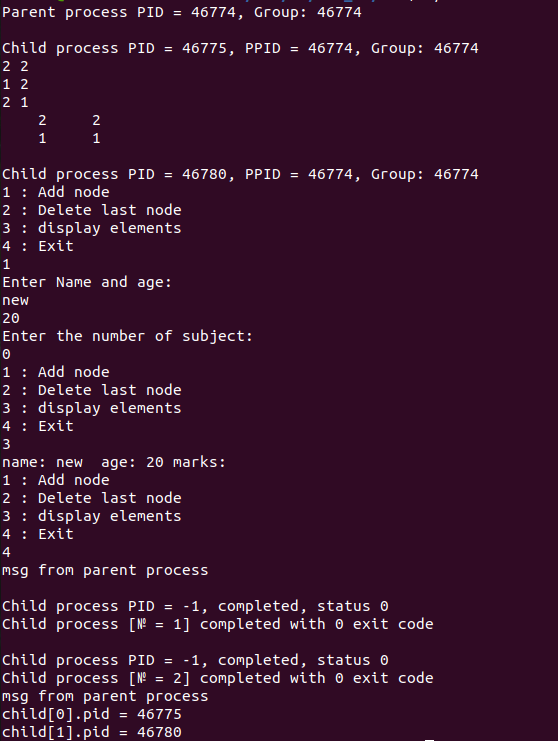
\includegraphics[width=\linewidth]{img/task03.png}
	\caption{Демонстрация работы программы (задание No3).}

	\label{fig:task03}

\end{figure}

\section*{Задание No4}

Предок и потомки обмениваются сообщениями через неименованный
программный канал. Предок ждет завершения своих потомков. Вывод соответствующих сообщений на экран.

\begin{lstlisting}[label=some-code,caption=Использование pipe,language=C]
#include <stdio.h>
#include <unistd.h>
#include <string.h>
#include <sys/wait.h>
#include <sys/types.h>

#define REP_N 2 // loop rep time
#define SLP_T 2 // sleep time
#define BUF_SIZE (sizeof(char) * 256)

enum error_code {
    ok,
    pipe_error,
    exec_error,
    fork_error,
    error
};

void read_message(const int *fd, char *buff, const int _end, const int _begin) {
    close(fd[_end]);
    
    int index = 0;
    
    while (read(fd[_begin], &buff[index++], 1) != 0) { }

    buff[index] = '\0';
}

int main()
{
    int child[REP_N], fd[REP_N];
    char buffer[BUF_SIZE];
    char *const msg[REP_N] = {"1st msg\n", "2nd msg long\n"};
    int pid;

    if (REP_N < 2) {
        perror("at most needs to create two childs!");
        return error;
    }

    if (pipe(fd) == -1) {
        perror("can't pipe!");
        return pipe_error;
    }

    printf("Parent process PID = %d, Group: %d\n", getpid(), getpgrp());

    for (size_t i = 0; i < REP_N; i++) {
        pid = fork();

        if (pid == -1) {
            perror("Fork failed!");
            return fork_error;
        } else if (pid == 0) {
            
            close(fd[0]);
            write(fd[1], msg[i], strlen(msg[i]));
            printf("msg No%zu sent from child to parent!\n", i + 1);

            return ok;
        } else {
            child[i] = pid;
        }
    }

    puts("msg from parent process");
    
    read_message(fd, buffer, 1, 0);
    printf("Received msg: \n%s\n", buffer);

    for (size_t i = 0; i < REP_N; i++) {
        int status, ret_val = 0;

        pid_t child_pid = wait(&status);

        printf("\nChild process PID = %d, completed, status %d\n", \
                                    child_pid, status);
        
        if (WIFEXITED(ret_val)) {
            printf("Child process [No = %zu] completed with %d exit code\n", 
                                        i + 1, WEXITSTATUS(ret_val));
        } else if (WIFSIGNALED(ret_val)) {
            printf("Child process [No = %zu] completed with %d exit code\n", 
                                        i + 1, WTERMSIG(ret_val));
        } else if (WIFSTOPPED(ret_val)) {
            printf("Child process [No = %zu] completed with %d exit code\n", 
                                        i + 1, WSTOPSIG(ret_val));
        }
    }

    puts("msg from parent process");
    
    for (size_t i = 0; i < REP_N; i++)
        printf("child[%zu].pid = %d\n", i, child[i]);
    
    return ok;
}
\end{lstlisting}

\begin{figure}[H]

	\centering

	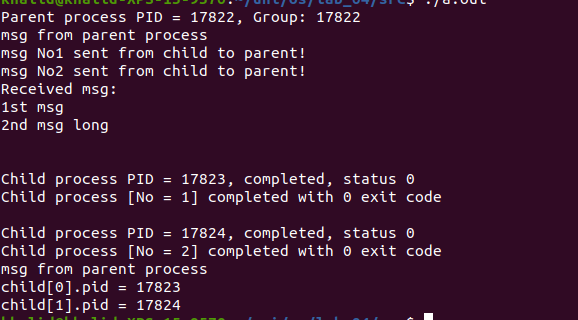
\includegraphics[width=\linewidth]{img/task04.png}
	\caption{Демонстрация работы программы (задание No4).}

	\label{fig:task04}

\end{figure}

\section*{Задание No5}

Предок и потомки обмениваются сообщениями через неименованный программный канал. С помощью сигнала меняется ход выполнения программы. Предок ждет завершения своих потомков. Вывод соответствующих сообщений на экран.

\begin{lstlisting}[label=some-code,caption=Использование сигналов,language=C]
#include <stdio.h>
#include <unistd.h>
#include <string.h>
#include <sys/wait.h>
#include <sys/types.h>

#define REP_N 2 // loop rep time
#define SLP_T 2 // sleep time
#define BUF_SIZE (sizeof(char) * 256)
#define GET 1

enum error_code {
    ok,
    pipe_error,
    exec_error,
    fork_error,
    error
};

int mode = 0;

void sigint_catcher(int signum) {
    printf( "\nProccess Catched signal #%d\n", signum);
    printf("Sent any message to clihd!\n");
    mode = 1;
}
int main()
{
    int child[REP_N], fd[REP_N];
    char buffer[BUF_SIZE] = { 0 };
    char *const msg[REP_N] = {"1st msg\n", "2nd msg long\n"};
    int pid;

    if (REP_N < 2) {
        perror("at most needs to create two childs!");
        return error;
    }

    if (pipe(fd) == -1) {
        perror("can't pipe!");
        return pipe_error;
    }

    printf("Parent process PID = %d, Group: %d\n", getpid(), getpgrp());
    signal(SIGINT, sigint_catcher);

    for (size_t i = 0; i < REP_N; i++) {
        pid = fork();

        if (pid == -1) {
            perror("Fork failed!");
            return fork_error;
        } else if (pid == 0) {
            signal(SIGINT, sigint_catcher);

            if (mode) {
                close(fd[0]);
                write(fd[1], msg[i], strlen(msg[i]));
                printf("msg No%zu sent from child to parent!\n", i + 1);
            } else {
                printf("No signal sent!\n");
            }

            return ok;
        } else {
            child[i] = pid;
        }
    }

    puts("msg from parent process");
    
    for (size_t i = 0; i < REP_N; i++) {
        int status, ret_val = 0;
        
        pid_t child_pid = wait(&status);

        printf("\nChild process PID = %d, completed, status %d\n", \
                                    child_pid, status);
        
        if (WIFEXITED(ret_val)) {
            printf("Child process [No = %zu] completed with %d exit code\n", 
                                        i + 1, WEXITSTATUS(ret_val));
        } else if (WIFSIGNALED(ret_val)) {
            printf("Child process [No = %zu] completed with %d exit code\n", 
                                        i + 1, WTERMSIG(ret_val));
        } else if (WIFSTOPPED(ret_val)) {
            printf("Child process [No = %zu] completed with %d exit code\n", 
                                        i + 1, WSTOPSIG(ret_val));
        }
    }
    
    close(fd[1]);
    read(fd[0], buffer, BUF_SIZE);
    printf("Received msg: \n%s\n", buffer);

    puts("msg from parent process");
    
    for (size_t i = 0; i < REP_N; i++)
        printf("child[%zu].pid = %d\n", i, child[i]);
    
    return ok;
}
\end{lstlisting}

\begin{figure}[H]

	\centering

	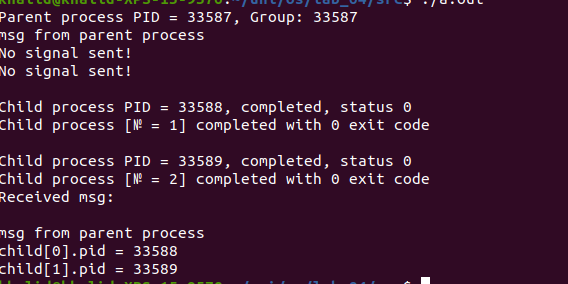
\includegraphics[width=\linewidth]{img/task05_01.png}
	\caption{Демонстрация работы программы, сигнал не вызывается (задание No5).}

	\label{fig:task05_01}

\end{figure}

\begin{figure}[H]

	\centering

	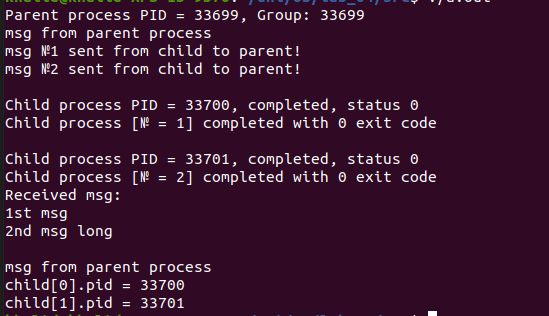
\includegraphics[width=\linewidth]{img/task05_02.png}
	\caption{Демонстрация работы программы, сигнал вызывается (задание No5).}

	\label{fig:task05_02}

\end{figure}


\bibliographystyle{utf8gost705u}  % стилевой файл для оформления по ГОСТу

\bibliography{51-biblio}          % имя библиографической базы (bib-файла)


\end{document}
